
\documentclass{beamer}
\usepackage{xparse}
\usepackage[latin1]{inputenc}
\usepackage{slashed}
\usepackage{amsmath}

\usepackage{amssymb}
\usepackage{amsfonts}
\usepackage{lmodern}
\mode<presentation> 
\usetheme{CambridgeUS}
\usepackage[english]{babel}
\usepackage{hyperref}
\usepackage{tabularx}
\usepackage{verbatim}
\usepackage{caption}
\captionsetup[figure]{labelformat=empty, font=tiny}% redefines the caption setup of the figures environment in the beamer class.



\begin{document}
\setbeamertemplate{bibliography item}{\insertbiblabel}
\title{Assignment 4}
\subtitle{Deep learning for image analysis}
\author{Adam, Smith, Jane \& Jessie}

\maketitle

%-----EXAMPLE SLIDES-----%

\begin{document}
\setbeamertemplate{caption}{\raggedright\insertcaption\par}
\begin{frame}
\frametitle{Introduction}
\begin{columns}
\begin{column}{0.5\textwidth}
\begin{itemize}
  \item Something
  \begin{itemize}
    \item Other things
    \item More things
    \item Something else
  \end{itemize}
\end{itemize}
\end{column}
\begin{column}{0.5\textwidth}  %%<--- here
\begin{center}
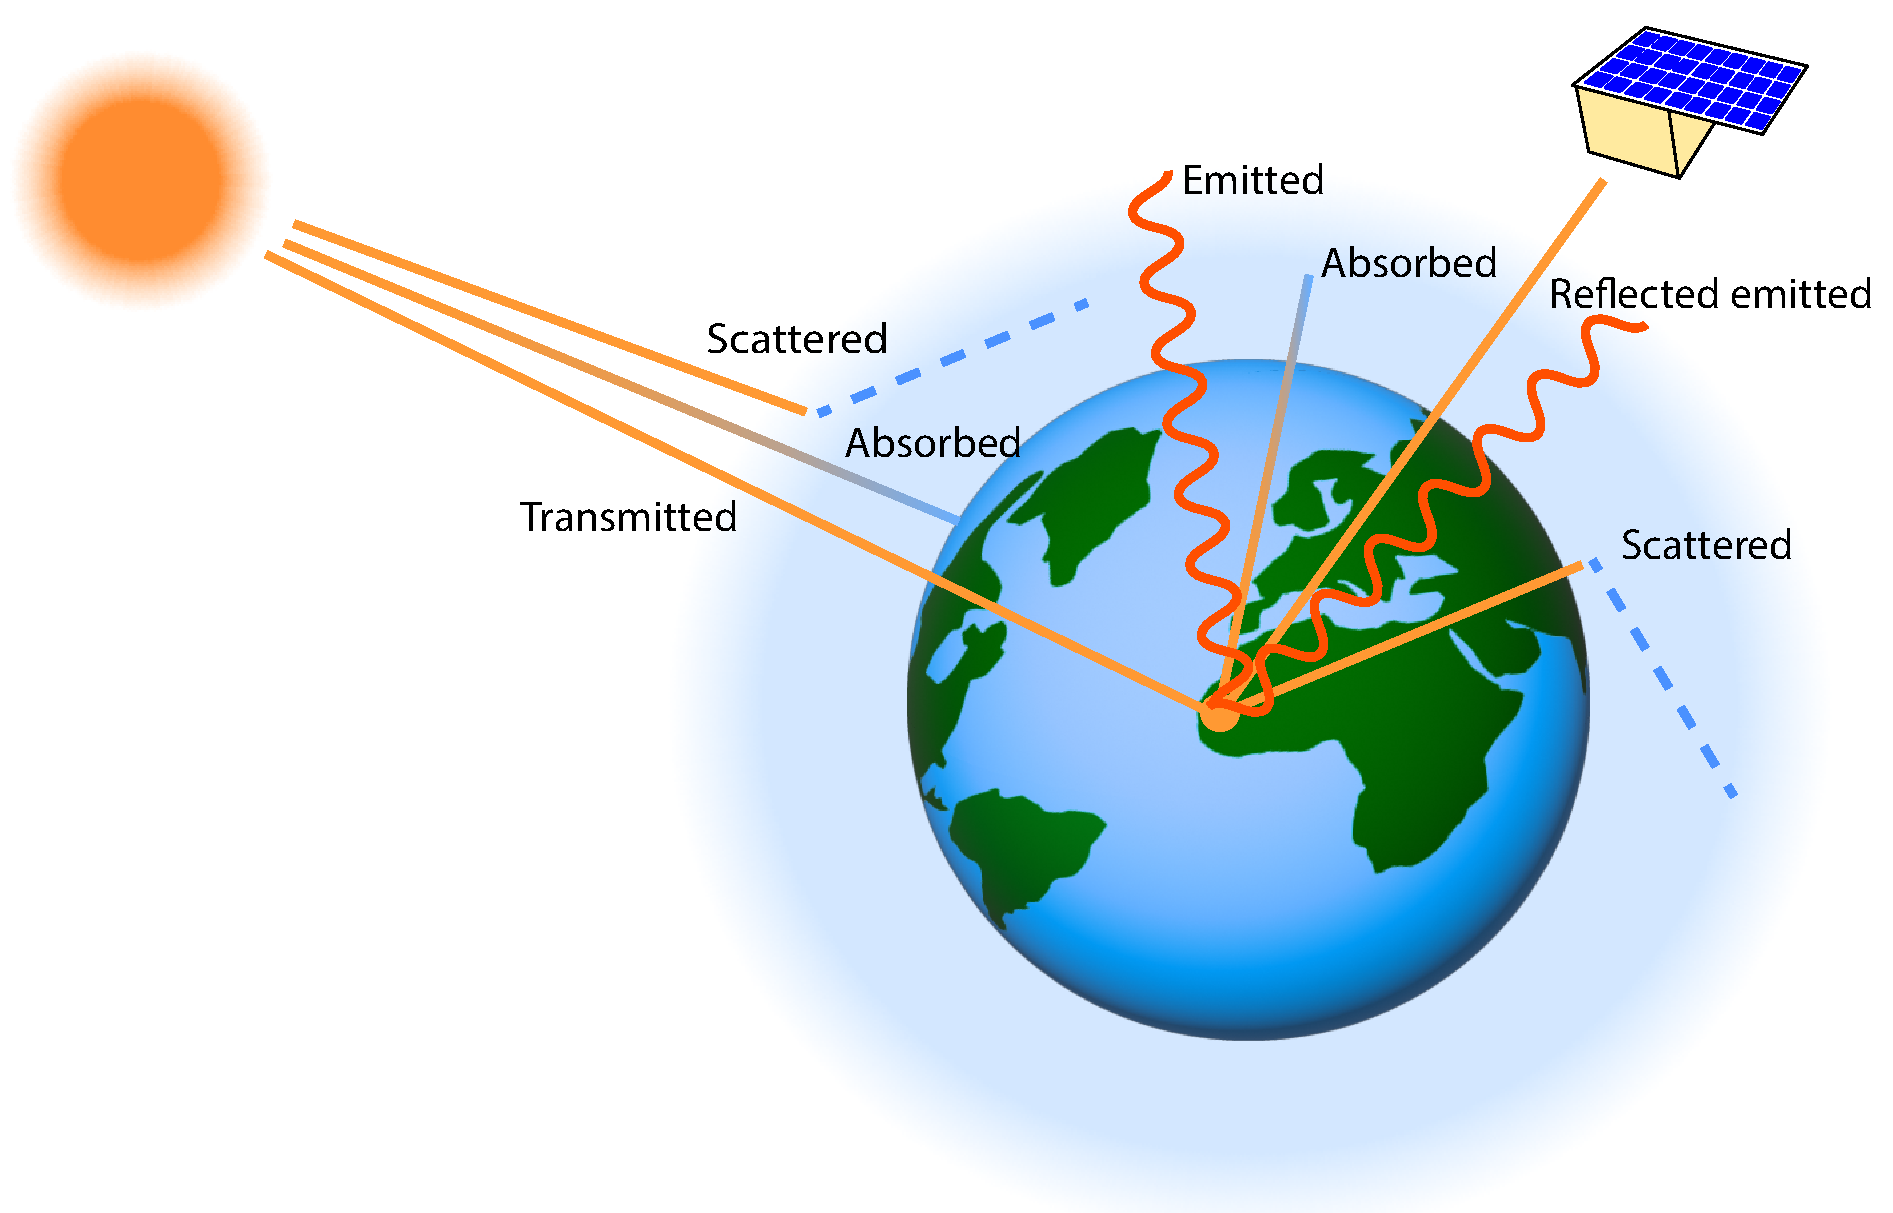
\includegraphics[width=1\textwidth]{figures/introduction_IIb.pdf}
\end{center}
\end{column}
\end{columns}
\end{frame}


% ------------------------------------------------- %

\begin{frame}[allowframebreaks] 
\frametitle{References}
\bibliographystyle{unsrt}
\bibliography{bibliography}


\end{frame}


\end{document}


%falcon9 https://commons.wikimedia.org/wiki/File:SpaceX_Falcon_9_rocket_and_Crew_Dragon_spacecraft_lifts_off_from_Launch_Complex_39A.jpg
% cubesats https://commons.wikimedia.org/wiki/File:ISS-38_Nanosatellites_deployment_(a).jpg
% temporal https://commons.wikimedia.org/wiki/File:ISS-40_Thunderheads_near_Borneo.jpg
% stressed plant https://commons.wikimedia.org/wiki/File:Starr-120504-5544-Kanaloa_kahoolawensis-leaves_showing_stress-nursery-Maui_(24511549154).jpg#filelinks
